\documentclass[10pt,letterpaper]{article}
\usepackage[letterpaper,hmargin=0.95in,vmargin=0.7in,footskip=22pt]{geometry}
\linespread{1.0}
\usepackage[T1]{fontenc}
\usepackage{XCharter}
\usepackage{fontspec}
\setmonofont{FiraMono-Regular.otf}[Scale=0.82]
\usepackage{microtype}
\usepackage{booktabs,array,tabularx}
\usepackage{graphicx}
\usepackage{float}
\usepackage[font=small,labelfont=bf,skip=6pt]{caption}
\usepackage{enumitem}
\usepackage{xcolor}
\usepackage{titlesec}
\usepackage[most]{tcolorbox}
\usepackage[hidelinks]{hyperref}

\definecolor{ink}{HTML}{0B0B0B}
\definecolor{soft}{HTML}{52514E}
\definecolor{rule}{HTML}{C3C2B7}
\definecolor{boxback}{HTML}{F4F3EE}

\setlength{\parindent}{0pt}
\setlength{\parskip}{5pt plus 1pt minus 1pt}
\setlist{itemsep=2pt,topsep=3pt,parsep=2pt,leftmargin=1.4em}
\titleformat{\section}{\large\bfseries}{\thesection}{0.6em}{}
\titleformat{\subsection}{\normalsize\bfseries}{\thesubsection}{0.6em}{}
\titlespacing*{\section}{0pt}{12pt plus 2pt minus 2pt}{4pt}
\titlespacing*{\subsection}{0pt}{9pt plus 2pt minus 1pt}{2pt}
\renewcommand{\arraystretch}{1.15}
\newcommand{\s}[1]{\texttt{#1}}          % a sentence or word of the toy language
\newtcolorbox{keybox}{colback=boxback,colframe=rule,boxrule=0.5pt,arc=2pt,
  left=8pt,right=8pt,top=6pt,bottom=6pt}

% generated


\begin{document}

\begin{center}
{\LARGE\bfseries Does a bigger vocabulary need a bigger model?}\\[5pt]
{\large Report on the experiments of the night of 21 to 22 November 2026}\\[3pt]
{\small\color{soft} Prepared by Claude. Every result in this report comes from runs saved in the folder \s{air}.}
\end{center}

\begin{keybox}
\textbf{The answer in short.} You asked whether a model that is kept the same size does worse
when its language has more words. I trained small models on a made-up language about animals,
with 16 to 1,024 animal words. The models came in four sizes, which I call widths 4, 8, 16 and
32. Each was graded on how many facts about the animals it knew, on a score from 0 (no better
than guessing) to 100 (every fact right).

\textbf{The verdict by the rule we fixed in advance: undecided.} The rule asks for a model
that learns the small language, comes to a stop clearly lower on a larger one, and is beaten
there by a model twice as wide. No model did that. One came close (point 5), but by the
test we fixed for it none of its runs had stopped improving when their time ran out. (The rule could only ever come out in favor of your idea or undecided.)

\begin{enumerate}[itemsep=1pt,topsep=2pt]
\item \textbf{The planned experiment did not put your idea to the test} (section
      \ref{sec:round1}). Widths 8, 16 and 32 each learned every fact of every language, from 16
      animals to 1,024, in all 36 runs. By a rough guide none of them was much more than
      one-third full, so there was nothing for more words to push out. What more words did
      cost was training: 64 times as many animals took about 6 to 8 times as much text.
\item \textbf{Using some animals far more often than others did no harm} (section
      \ref{sec:zipf}). All 36 runs were solved again, and the large languages were learned
      sooner than with equal use.
\item \textbf{Part-way through training, the scores look like your prediction} (section
      \ref{sec:equal}). This is the comparison you suggested: every model after the same
      amount of text. At one such point width 16 scored 100 on 16 animals but only 59 on 256
      animals, and width 32 scored 81 on those 256. But the cause is not the one your idea
      names. Your idea is about room; this is about speed. A larger language takes more text
      to learn and a wider model learns it from less, and with more text every one of these
      models reached 100.
\item \textbf{The claim your idea starts from, that a model stores what words mean, is
      supported} (section \ref{sec:probe}). Each word has a row of numbers of its own in the
      model. A simple test could read an animal's facts from its row 70 to 97 times in 100,
      and animals with the same facts ended up with nearly the same row.
\item \textbf{The nearest thing to your prediction came when each animal had 16 facts in
      place of 4} (section \ref{sec:round32}). Widths 8, 16 and 32 all still learned the 16
      animals. On 256 animals widths 16 and 32 learned practically everything too, but width 8
      did not. In three runs it stayed below 60, and in the two that got furthest it held only
      about two of the four kinds of fact. That is what a model too small for its language would
      look like. One night was not enough to tell it apart from a model that is only very slow.
\item \textbf{Runs can stand still for a long time and then go on} (section
      \ref{sec:round32}). In that same round two models stood at a score of 37 for so long
      that our test for the end of a run called them finished. I replayed one of them exactly
      and let it run four times as long: it stood at 37 for most of that time and then rose
      to 98.6. The other I started again from the same numbers on the same text, with the
      computer set up slightly differently, which changes only the last digits of its
      arithmetic. It never paused at 37 and reached 100. Whether a run got stuck was chance.
\item \textbf{The smallest model, width 4, learned no facts in the time it had} (section
      \ref{sec:four}), not even about 16 animals, though it learned the shapes of the
      sentences. It seems too narrow to work at all, which would be a different thing from
      being too full.
\end{enumerate}

\textbf{Two lessons.} First, because every word has a row of its own, each added word brings
room with it. That is the likely reason why adding words alone did not fill a model here. To
test your prediction properly, the words must be made to share one store of fixed size;
section \ref{sec:extras} says how. Second, these models learn in jumps, with long stand-stills
in between. A model that has stopped improving is not necessarily finished.
\end{keybox}

\section{The idea}

Your idea is that a language model is a store of what words mean. A store of a given size can
hold only so much. So a language with few words should need only a small model, and a model
that is kept the same size should do worse when it is given a language with more words, once
the words no longer fit.

To test this we need a language in which we control the number of words exactly and know every
right answer, so that a model can be graded without doubt. No real language allows that, so we
made one up. In it, ``what a word means'' is something we can write down: a short list of facts
about the thing the word names.

\section{The made-up language}

The language is about animals. Its smallest version has 43 words:

\begin{quote}\small
16 animals: \s{foxes bears wolves owls bats frogs snakes crows}\\
\phantom{16 animals: }\s{hens ducks deer mice toads robins otters lizards}\\
4 colors: \s{red brown green black}\qquad 4 foods: \s{meat plants insects seeds}\\
4 homes: \s{woods fields rivers caves}\qquad 4 waking times: \s{dawn noon dusk night}\\
11 sentence words: \s{are do eat live in wake at yes no . ?}\quad (the full stop and the question mark count as words)
\end{quote}

Each animal has four facts: its color, its food, its home and the time it wakes. Each fact has
one of four values. For example, foxes are red, eat meat, live in woods and wake at dusk. Those
four facts are what the word \s{foxes} means in this language.

There are two kinds of sentence. A \emph{statement} gives one fact. A \emph{question} asks
whether a fact has a certain value and is followed by yes or no:

\begin{quote}\small
\s{foxes are red .}\qquad \s{foxes eat meat .}\qquad \s{foxes live in woods .}\qquad
\s{foxes wake at dusk .}\\
\s{do foxes eat meat ? yes}\qquad \s{do foxes eat seeds ? no}
\end{quote}

Every statement is true and every yes or no is right. The text a model learns from is simply
these sentences one after another, in random order: six in ten are statements and four in ten
are questions. The questions are there so that the language is more than one sentence shape
repeated. The score in this report uses statements only.

\textbf{A larger language} has more animals: 64, 256 or 1,024 in place of 16. The added animals
have invented names (\s{bakos}, \s{gigas}, \s{vofos}, \dots) and invented facts. The facts are
drawn at random, but evenly: a quarter of the animals are red, a quarter brown and so on, and
the same for food, home and waking time. The first 16 animals are the same in every language
and are spread just as evenly. Nothing else differs between the languages: the sentences have
the same shapes and the 27 words that are not animals are the same.

\textbf{Counting how much there is to know.} To say how full a model is, we need a measure of
how much a language asks it to remember. We count in \emph{bits}: one bit is what it takes to
settle a choice between two things, and a choice among four takes two bits. So one fact counts
as 2 bits and an animal, with its four facts, as 8 bits. This is the same for every animal in
every language, as you insisted: a large vocabulary must differ from a small one only in the
number of words, not in how much each word means. A whole language holds 8 bits times its
number of animals: 128 bits for 16 animals, 8,192 for 1,024.

\section{The model and how it learns}\label{sec:model}

A model is a long list of numbers together with a fixed recipe for using them. Given the words
read so far, the recipe produces, for every word of the language, how likely that word is to
come next. The numbers are called \emph{parameters}. At the start they are random, so the
model's predictions are worthless.

\textbf{Training.} The model is given a stretch of text, about 1,160 sentences. At each word it
says how likely every word is to come next, and this is compared with the word that really
comes next. Then all its numbers are changed a little, in the direction that would have made
the real next words more likely. That is one \emph{training step}.

\textbf{The two parts of a model.} The \emph{word table} holds one row of numbers for each
word. The \emph{body} takes the rows of the words read so far and works out the prediction.
The count of numbers in one row is called the \emph{width}: a model of width 8 keeps 8 numbers
for each word. The body is built from pieces of the same width, so a wider model has a larger
body too. Width is the only thing we changed to make a model smaller or larger. We used widths
4, 8, 16 and 32 (table \ref{tab:sizes}). For scale, the models behind chat assistants have
billions of parameters.

\textbf{The same count of numbers for every language, but not the same amount in use.}
Normally a model built for more words would be bigger, because it would need more rows. To
prevent that, every model has a row for each of the 1,024 animals, whichever language it is
trained on, so a model of width 8 always has 10,936 parameters. This only half works. A model
trained on 16 animals never reads the other 1,008 animal words, so their rows lie idle. In
effect it is a smaller model, with its body and 43 rows: about 2,900 numbers at width 8. A model
trained on 1,024 animals uses all 10,936. So every added animal arrives with a row of its own,
8 numbers at width 8, in which its facts could be kept. The only part that is truly the same
size for every language, and that all the animals share, is the body. This matters for reading
the results: if a model learns a larger language without trouble, that may be because each
new animal brought its own row, and not because the model had room to spare. Section
\ref{sec:meaning} comes back to this.

\begin{table}[H]
\centering\small
\begin{tabular}{@{}rrrrcc@{}}
\toprule
Width & \multicolumn{3}{c}{Number of parameters} & Bits of facts per parameter & How full, against \\
 & in the body & in the word table & in all & with all 1,024 animals & a limit of 2 bits \\
\midrule
4 & 880 & 4,204 & 5,084 & 1.61 & about 80\% \\
8 & 2,528 & 8,408 & 10,936 & 0.75 & about 37\% \\
16 & 8,128 & 16,816 & 24,944 & 0.33 & about 16\% \\
32 & 28,544 & 33,632 & 62,176 & 0.13 & about 7\% \\
\bottomrule
\end{tabular}
\caption{The four model sizes. The word table has 1,051 rows in every model: 27 for the words
that are not animals and 1,024 for the animals. The fifth column is the 8,192 bits of the
largest language divided by the model's number of parameters. The last column compares that
with the rough limit of 2 bits per parameter explained below.}
\label{tab:sizes}
\end{table}

\textbf{How full can a model get?} A study of much larger models of this kind (Allen-Zhu and
Li, 2024; a million to several hundred million parameters) found that a model holds at most
about 2 bits of facts per parameter. Nobody has measured this for models as small as ours, so
2 is only a rough guide. By that guide \emph{none} of our models should be full with 8 bits
per animal: width 4 would be about four-fifths full if it learned all 1,024 animals, width 8 a
little over one-third full, and the two widest far emptier. We could see this before the runs.
I ran the plan all the same, because it is the experiment we agreed and because the guide
might not hold for models this small.

\textbf{Three rounds.} We had agreed on three rounds of runs. The \emph{first round} is the
plan as described so far (section \ref{sec:round1}). The \emph{unequal-use round} repeats it
with some animals mentioned far more often than others (section \ref{sec:zipf}). The
\emph{32-bit round} gives each animal four times as much to be known (section
\ref{sec:round32}); it was to be run only if the first round supported your idea.

\section{Keeping the comparison fair}

When the vocabulary grows, nothing else should change, or a worse score could be blamed on
whatever else changed. Two safeguards are already described: every animal carries the same
number of bits, and every model has the same count of numbers whatever the language (though,
as just explained, a larger language puts more of them to use). There are two more.

\textbf{The text is dealt out in equal portions, which we called sets.} A set is always 61,440
sentences, whatever the language. That is what it takes to bring up each of the 4,096 facts of
the largest language 15 times: nine times as a statement, three times in a question answered
yes, and three times in a question answered no. In the first round a set brings up each fact
exactly as often as every other fact, in every language, and each new set is the same sentences
in a new random order. One set is 53 training steps.

\textbf{One more thing changes with the vocabulary, and it cannot be avoided.} A set is the
same length for every language. In the largest language it brings up each fact 15 times. The
smallest language has 64 times fewer facts, so there each fact comes round 960 times in a
set. You pointed out that this is what a larger vocabulary is: each word gets a smaller share
of everything that is said. So that this does not decide the result, the planned comparison is
not made after equal numbers of sets. Each run goes on receiving sets until more training no
longer raises its score, or until its time runs out (next section). Section \ref{sec:equal}
makes the other comparison as well.

\section{The score, and how a run ends}\label{sec:score}

\textbf{The score} is called \emph{facts known}. The model is given the start of a statement,
such as \s{foxes eat}, and nothing else: no earlier sentences it could copy from. If the word
it rates most likely to come next is the right one (\s{meat}), the fact counts as known. This
is done for every fact of every animal in the language. It is a test of memory, on purpose:
the facts were all in the training text, and the question is whether the model has kept them.

A model that knows nothing can still be right one time in four, by always giving the same
value. The score is set up to remove that luck: \textbf{0 stands for one fact in four right,
which is no knowledge at all, and 100 for every fact right.} In between, a score of 90 means
92.5 facts in 100 are right.

A \emph{run} is one model trained on one language. It is graded often at first and then less
and less often: after 1, 2, 3, 4, 6, 8, 11, 16 sets and so on, so that every second grading
comes after about double the training. A run ends in one of three ways, and which way it ends
decides what it can tell us.
\begin{itemize}
\item \textbf{Solved.} The score was 97 or more at two gradings in a row. The model is big
      enough for this language.
\item \textbf{Flat.} The score has stopped rising: doubling the training added less than 2
      points, and doubling it again also added less than 2 points. (An invented example: 70
      after 256 sets, 71 after 512, 71.5 after 1,024.) Before a run is called flat, three more
      things must hold. A second, finer measure, how well the model predicts the next word of
      a text, must have stopped improving too. The score must be at least 5. And the run must
      be past its start: at least 2,000 training steps (about 38 sets in the first round),
      with each fact brought up at least 400 times. The score of a flat run was to be taken as
      the model's limit on that language. Section \ref{sec:round32} shows that this trusted
      the test too much.
\item \textbf{Not finished.} The time allowed ran out first. The time limit is a safety net so
      that one run cannot take the whole night: 30 minutes in the first round, which is a
      little over 1,600 sets. When its time is up a run is graded one last time. If that makes two gradings
      of 97 or more in a row, it counts as solved. Otherwise it is not finished: it tells us
      nothing about the model's limit, and I draw no conclusion about that limit from it.
\end{itemize}
The marks 97 and 2 points here, and the 95 and 10 points of the rule below, are judgment calls
that were fixed before any run. The mark of 5 and the 2,000 steps were added later, but
before the real runs (section \ref{sec:changes}).

\section{The rule we fixed in advance}\label{sec:rule}

Each pairing of a width and a language was to be run three times. I call these the three
\emph{repeats}. They differ in the random starting numbers of the model, in the order of the
sentences, and in the invented facts of the added animals. Within one repeat, models of all
widths read exactly the same text.

Before any run we agreed what would count as clear support for your idea. The rule looks at
one width at a time. In one repeat, that width counts in favor of the idea if all three of
these hold:
\begin{enumerate}[label=(\alph*),leftmargin=2.2em]
\item On the 16-animal language the model scores 95 or more. So it can learn the small language.
\item On one of the larger languages its run ends \emph{flat}, with a score at least 10 points
      below its own score on 16 animals. So it does worse with more words, and not because
      it was stopped early.
\item On that same language, in the same repeat, the model twice as wide scores at least 10
      points higher than this model. So a bigger model wins back what was lost, which points
      to size as the cause.
\end{enumerate}
The idea is clearly supported for that width if this happens in at least two of its three
repeats.

We also agreed how to read the other outcomes. If a model does worse on a larger language but
the model twice as wide does no better, something other than size is holding it back. If no
model does worse on any larger language, the round has not tested the idea: the idea says that
more words hurt once the model is full, and nothing shows that any model was full.

Notice what this means: \textbf{the rule can come out in favor of your idea, or undecided,
but never against it.} We agreed on nothing that would show the idea wrong. The nearest thing
would be a model that ought to be nearly full by the guide of 2 bits per parameter and still
learns every fact, and even that would be weak evidence, because the guide is rough.

\section{What trial runs changed before the experiment}\label{sec:changes}

Before the real runs I made short trial runs to check that the set-up works. They led me to
change three things without asking you (points 1, 3 and 4) and showed one thing I had not
expected (point 2). The rule itself is untouched. But point 3 changes how a model is graded and
point 4 changes when a run may be called flat, and the rule depends on both.

\textbf{1. The speed of learning.} A setting called the learning rate decides how strongly the
numbers are changed at each step. My first value was too cautious: with a value five times
higher, width 8 learned the 16 animals about six times sooner. I chose the value using the
16-animal language only, so that I could not, even without meaning to, pick one that gave a
particular result on the large languages. Every width and every language used that one value.

\textbf{2. In the trial runs the smallest model learned no facts.} Width 4 learned the shapes
of the sentences, but its score was still 0 after 360 sets, even with only 16 animals (section
\ref{sec:four}). A width that fails condition (a) cannot count in favor of your idea, and
width 32 cannot either, because condition (c) needs a model twice as wide. So in the first
round the rule could only be met for widths 8 and 16.

\textbf{3. The score wobbled, so I grade a steadied copy of the model.} With the higher
learning rate, the numbers of a small model on a large language keep shifting a little at every
step, and the score shifts with them. In a trial run of width 8 on 1,024 animals, four gradings
in a row gave 97.6, 96.5, 91.9 and 100.0: a swing of 8 points, too much for a rule that turns on
10. The standard cure is to keep, beside the model being trained, a second copy in which each
number is the average of what that number has been over the last few hundred steps, and to
grade that copy. The training itself is not changed. To see what difference this makes I
repeated one such run without it. The model learned the language just the same, but its score
went on swinging: 96.1, 99.8 and 95.8 at three gradings in a row, so it did not pass the test
for ``solved'' (97 or more twice running) in the 397 sets I gave it. The steadied copy had
scored 100 and 100 at the first two of those gradings. One side effect of the copy: it is always a little
behind the model being trained, by roughly ten sets in the first round.

\textbf{4. A model can look finished before it has begun.} A model first learns the sentence
shapes, then stands still for a while with a score of zero, and only then starts to learn
facts. The ``flat'' test could not tell that pause from a model at its limit: it ended one trial
run, width 16 on 1,024 animals, as flat with a score of 0.4, although that width later learned
every fact of that language. A false ``flat'' on a large language is exactly what condition (b)
looks for, so this could have produced false support for your idea. Two conditions now
guard against it: a run cannot be called flat in its first 2,000 training steps (added when the
programs were reviewed), nor while its score is below 5 (added after this trial run).
A run that never starts to learn facts now ends as ``not finished''. The cost: a model that
truly cannot learn anything of a large language now looks the same as one that needs more time. Even so
repaired, the test was fooled once more, by a later and longer pause (section
\ref{sec:round32}).

\textbf{Checking the programs.} The programs that write the sentences and grade the models
were checked before use by other copies of Claude, the AI that wrote this report, each working
from the programs alone. They confirmed that every sentence is true, that each set holds
exactly the agreed number of each fact, and that a made-up ``model'' which knows everything is
graded 100 and one which knows nothing is graded 0.

\section{Result 1: with 8 bits per animal, no model ran out of room}\label{sec:round1}

This is the first round, without width 4: the four languages (16, 64, 256 and 1,024 animals),
three widths (8, 16 and 32) and three repeats of each pairing, 36 runs in all. In the trial
runs width 4 had still learned no facts after 360 sets, even on 16 animals, so I ran it
separately (section \ref{sec:four}). That is a loss for the test: by the rough guide width 4 was
the one size that would have come near full on 1,024 animals.

\begin{table}[H]
\centering\small
\begin{tabular}{@{}rrrrr@{}}
\toprule
 & \multicolumn{4}{c}{Animals in the vocabulary} \\
Width & 16 & 64 & 256 & 1{,}024 \\
\midrule
8 & 100 & 100 & 100 & 100 \\
16 & 100 & 100 & 100 & 100 \\
32 & 100 & 100 & 100 & 100 \\
\bottomrule
\end{tabular}

\caption{Facts known (0 to 100) at the end of each run, with 8 bits per animal. Each entry
covers three repeats; a single number means all three gave that score.}
\label{tab:round1}
\end{table}

\textbf{All 36 runs ended as solved, with a score of 100} (table \ref{tab:round1}). A model of
width 8 learned all 4,096 facts about 1,024 animals as completely as it learned the 64 facts
about 16 animals.

Remember the catch from section \ref{sec:model}: this was not one store of fixed size taking
in 64 times as much. Every added animal came with a row of its own, and only the body was the
same size in both.

\textbf{Verdict of this round: undecided}, as section \ref{sec:rule} said it would be if no
model did worse. The rule is not met for width 8 or for width 16, the two widths it could be
met for. That is not evidence against your idea, because the idea predicts a loss only once
the words no longer fit, and by the rough guide the fullest of these models (width 8 on 1,024
animals) was a little over one-third full. What the round does show is narrower: with room to
spare, 64 times as many words did not leave any of these models worse off at the end of its
training.

\textbf{What a larger vocabulary did cost was training time.} Table \ref{tab:effort1} shows
how many sets each run had read when it was declared solved.

\begin{table}[H]
\centering\small
\begin{tabular}{@{}rrrrr@{}}
\toprule
 & \multicolumn{4}{c}{Animals in the vocabulary} \\
Width & 16 & 64 & 256 & 1{,}024 \\
\midrule
8 & 64, 64, 91 & 64, 91, 181 & 256, 256, 512 & 256, 512, 1{,}639 \\
16 & 32, 32, 32 & 45, 45, 64 & 64, 64, 91 & 128, 181, 181 \\
32 & 16, 23, 23 & 23, 32, 32 & 64, 64, 64 & 91, 128, 128 \\
\bottomrule
\end{tabular}

\caption{Sets of training text read before each run was solved, for the three repeats,
smallest first. Runs are graded only after certain numbers of sets and must pass twice in a
row, so these figures move in jumps, and two equal figures may hide a real difference. The
figure 1,639 is the one run that was graded because its time had run out.}
\label{tab:effort1}
\end{table}

Two things stand out.

\textbf{More words took more sets, but far fewer than in proportion.} From 16 to 1,024 animals
there are 64 times as many facts. Taking the middle one of the three figures in each entry of
table \ref{tab:effort1}, width 8 needed 8 times as many sets (512 against 64), and widths 16
and 32 needed about 6 times as many.

\textbf{The smaller the model, the more sets it needed, and the less dependable it was.} On
1,024 animals, width 8 needed four times as many sets as width 32 (512 against 128, the middle
figures), and its
three repeats differed widely: 256, 512 and 1,639 sets. The slowest only just made it: it
passed for the second time at the grading made when its 30 minutes ran out. For its first 250 sets its score stayed near zero. Later it stood still
again, at a score of 25 from set 512 to set 724, before climbing to 52 and then to 100. (A
score of 25 is what a model gets if it knows one of the four kinds of fact for every animal, so
it seems to have picked up one kind of fact at a time.) This is a warning for everything that
follows: a model can stand still for a long time and then move again.


\section{Result 2: unequal use of the animals did no harm}
\label{sec:zipf}

You pointed out that in real language words are not used equally often, and that this is part
of what a language is. So the first round was run again with unequal use: the most
common animal is mentioned twice as often as the second, three times as often as the third,
and so on down the list. The 16 original animals are the most common ones. With 1,024 animals
they get 45\% of all mentions, and the rarest animal is mentioned 7.5 times less often than it
would be with equal use. These are again 36 runs. To fit the night I cut the time limit from 30
minutes to 5, roughly 270 sets. That turned out not to matter: every run was solved inside it,
the slowest after 256 sets.

\textbf{All 36 runs ended as solved.} The lowest score was 99.1. So the rule is again not met
for any width, and for the same reason: no model ended up worse with more words.

\textbf{The large languages were learned in fewer sets than with equal use.} On 1,024 animals
width 32 needed 45 sets in all three repeats, where it had needed about 128 (table
\ref{tab:effort1}). Width 8 needed 181, 181 and 256 sets, where it had needed 256, 512 and
1,639. The rare
animals were learned too. When width 32 was solved on 1,024 animals, each fact of the rarest
animal had come up only about 90 times. With equal use, each fact had come up more than 1,300
times before the same model was solved.

I had expected the opposite, that rare words would hold a model back. My explanation, which
these runs do not test: the common animals get a model past its early stand-still sooner, and
after that it needs far fewer showings to add another animal.

\section{Result 3: part-way through training, the scores look like your prediction}
\label{sec:equal}

While we were planning you suggested another way to compare: give every model the same amount
of text and then see how well it does, without waiting for each one to finish. We left that
for after the main experiment. It needs no new training. Every run was graded as it went
along, so I can read off what each model scored after the same number of sets, which is the
same amount of text in every language.

\begin{table}[H]
\centering\small
\begin{tabular}{@{}rrrrr@{\qquad}rrrr@{}}
\toprule
 & \multicolumn{4}{c}{After 32 sets} & \multicolumn{4}{c}{After 64 sets} \\
Width & 16 & 64 & 256 & 1{,}024 & 16 & 64 & 256 & 1{,}024 \\
\midrule
8 & 69 & 37 & 5 & 0 & 100 & 74 & 17 & 2 \\
16 & 100 & 97 & 59 & 13 & 100 & 100 & 100 & 51 \\
32 & 100 & 100 & 81 & 32 & 100 & 100 & 100 & 75 \\
\bottomrule
\end{tabular}

\caption{Facts known (0 to 100) after 32 sets and after 64 sets of text, by width and by the
number of animals in the language. First round, average of the three repeats. A run that was
already solved by then is entered with its final score. I show 32 and 64 sets because earlier
most entries are near 0 and later most are 100.}
\label{tab:equal}
\end{table}

\textbf{Part-way through training, the scores look like your prediction} (table
\ref{tab:equal}). Take width 16 after 32 sets. It scores 100 on 16 animals, 59 on 256 and 13 on
1,024: the more words, the lower the score. And a wider model scores higher. On 256 animals
after 32 sets, width 8 scores 5, width 16 scores 59 and width 32 scores 81. The unequal-use
round shows the same pattern: after 32 sets on 1,024 animals the three widths score 19, 79 and
99.

\textbf{But the cause is not the one your idea names.} Your idea is about room: a model that
is full cannot take in more words however long it is trained. Nothing here shows a full
model. With more text every one of these models went on to a score of 100 (section
\ref{sec:round1}). What the table shows is speed. A larger language takes more text to learn,
and a wider model learns it from less.

\textbf{A larger language needs more text in all, but less text for each fact.} In all: width
8 needed 512 sets for 1,024 animals against 64 sets for 16 (the middle one of its three repeats
each time), 8 times the text for 64 times the facts. For each fact: one set shows each fact of
the smallest language 960 times and each fact of the largest only 15 times. So by the time
width 8 was solved, each fact had come up about 61,000 times in the small language and about
7,700 times in the large one.

\textbf{How much weight to give this.} What the comparison shows is true and useful: with a
limited amount of text, the same model knows less of a larger language, and a wider model knows
more of it. What it cannot show is why. A model that has run out of room and a model that only
needs more text look the same at one moment in training. Here we know it was the second,
because with more text every model reached 100. And although you proposed the comparison, we
fixed no rule for reading it, and I chose the two moments in the table after seeing the
results. So it is an observation, not a test.

\section{Result 4: what a word means can be found in its row}\label{sec:probe}

Your idea starts from the claim that a model is a store of what words mean. In this language we
know exactly what each word means, so we can look for it inside a trained model. After training,
each animal has its own row of numbers in the word table. I asked two questions about the rows
of the nine models of the first round that had learned all 1,024 animals.

\textbf{Can a fact be read from a row?} I call this the read-out test. Take color. For each of
the four colors the test has a list of multipliers, one for each number in a row. It multiplies
each number of an animal's row by its multiplier and adds up the results; the color with the
largest total is its answer. The multipliers are worked out from half of the animals, whose
colors it is told. Then the test is tried on the other half, which it has never seen. If the
rows held no trace of color it would be right for about one animal in four.

\begin{table}[H]
\centering\small
\begin{tabular}{@{}rrrrrr@{}}
\toprule
Width & Color & Food & Home & Waking time & Facts shared with \\
 & & & & & the nearest row (of 4) \\
\midrule
8 & 71\% & 74\% & 70\% & 72\% & 3.98 \\
16 & 88\% & 84\% & 74\% & 83\% & 3.97 \\
32 & 97\% & 88\% & 97\% & 92\% & 3.98 \\
\bottomrule
\end{tabular}

\caption{Left four columns: how often the read-out test names the right value for animals it
was not worked out on, from their rows alone (average of the three repeats; guessing gives
25\%). Right column: how many of its four facts an animal shares with the animal whose row is
most like its own (two animals picked at random share 1.00).}
\label{tab:probe}
\end{table}

Table \ref{tab:probe} gives the result. The test is right for between 70\% and 97\% of the
unseen animals, far above guessing, and the wider the model the better. It is not right for all
of them, although the models themselves get every fact right. Either the rest is in the rows in a
form this very simple test cannot read, or part of it is kept in the body, which can tell an
animal by its row.

\textbf{Do animals with the same meaning sit together?} There are only 256 possible
combinations of four facts, and 1,024 animals, so nearly every animal has at least one other
animal with exactly the same four facts. For each animal I looked up the other animal whose
row is most similar: the one whose numbers are high where its own are high and low where its
own are low. Almost always it is one of those twins: the two share 3.97 or 3.98 of their 4 facts on average, where two animals
picked at random share 1. Nothing in the training text ever says that two animals are alike.
The model gave them nearly the same row because the same things are said about them.

\begin{figure}[H]
\centering
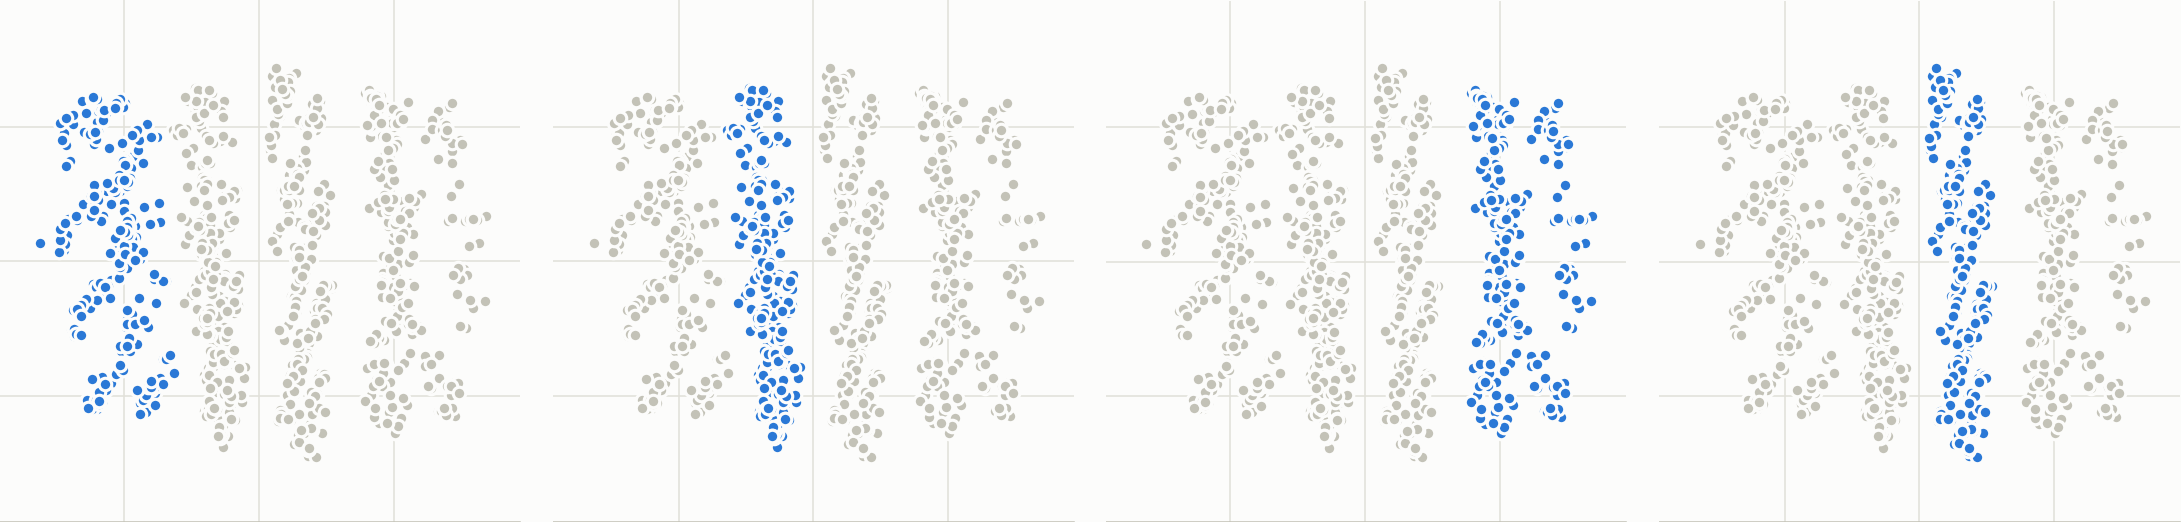
\includegraphics[width=0.74\textwidth]{figures/probe_strip.png}\\[1pt]
{\small\makebox[0.185\textwidth]{red}\makebox[0.185\textwidth]{brown}\makebox[0.185\textwidth]{green}\makebox[0.185\textwidth]{black}}
\caption{The rows of the 1,024 animals in one model of width 32. A row has 32 numbers, too many
to draw. So each row is squeezed down to two numbers, each a weighted sum of the 32, chosen as
the two sums that vary most from one animal to another. Each dot is one animal, placed by those
two numbers, so animals with similar rows land close together. The four panels show the same
dots; each colors in blue the animals of one color. They fall into four bands.}
\label{fig:probe}
\end{figure}

This supports the claim your idea starts from: in these models an animal's row is, to a large
extent, a description of what the word means. Animals that mean the same get nearly the same
row, and most of the meaning can be read out by a very simple test. It says nothing about size.

\section{Result 5: with 32 bits per animal, runs stood still so long that they looked finished}
\label{sec:round32}

The first round could not test your idea, because no model was full. The only way left to press
the models harder was the 32-bit round. We had agreed to run it only if the first round
supported the idea, which it did not. I ran it all the same, because you told me during the
night to run everything.

\textbf{What changed.} Each animal now has its four facts for each of four seasons: 16 facts
in place of 4, and 32 bits in place of 8. Four words are added (\s{winter spring summer fall}),
and every sentence begins with a season: \s{in winter foxes eat meat .} An animal's facts in one
season have nothing to do with its facts in another. Every animal in every language of this
round carries the same 32 bits. A set is now four times as long, so that it still brings up
each fact of the largest language 15 times.

\textbf{How full the models would be.} I count, as in section \ref{sec:model}, only the numbers
a model really uses: its body and the rows of the words of its own language. By the rough guide
a model that learned all 256 animals would then be 85\% full at width 8, about one-third full
at width 16 and about one-tenth full at width 32. (That is as many bits as the 1,024 animals
of the first round, where width 8 came to 37\%. It is fuller now because it has only 256 animal
rows to keep them in.) With 1,024 animals the figures are 149\%, 66\% and 26\%.

\textbf{With 16 animals nothing changed.} Widths 8, 16 and 32 learned every fact, in both
repeats that I ran, within 16 to 64 sets.

\textbf{With 256 animals, the first runs looked like a failure.} I ran the agreed procedure
once for each width (the lines marked ``first run'' in table \ref{tab:large}). Widths 16 and 32
rose quickly to a score of 37 and stayed there, and the stopping test ended them as flat. Width
8 rose slowly, passed them, and was at 59 when its time ran out. (Its limit was first 15
minutes, in which it reached 48 after 174 sets; I replayed it with 40 minutes, because it was
the one run still climbing.) For width 16 the first two parts of our rule held: it had learned the 16
animals, and on 256 animals its run ended flat at a far lower score. The third part failed:
the model twice as wide did no better, with the same 37. By our agreement that means something
other than size was holding width 16 back. (For width 32 the rule cannot be asked, because I
ran no width 64.)

\begin{table}[t]
\centering\small
\begin{tabular}{@{}rrlcrrl@{}}
\toprule
Animals & Width & Run & ``Flat'' ending & Sets & Facts known & How it ended \\
\midrule
256 & 8 & repeat 1, first run & on & 445 & 59.2 & time ran out \\
256 & 8 & repeat 1, run again & off & 776 & 44.1 & time ran out \\
256 & 8 & repeat 2 & off & 391 & 34.8 & time ran out \\
\addlinespace[2pt]
256 & 16 & repeat 1, first run & on & 128 & 37.3 & ended as flat \\
256 & 16 & repeat 1, run again & off & 512 & 98.6 & fixed length reached \\
256 & 16 & repeat 2 & off & 91 & 99.9 & solved \\
\addlinespace[2pt]
256 & 32 & repeat 1, first run & on & 91 & 37.2 & ended as flat \\
256 & 32 & repeat 1, run again & off & 64 & 100.0 & solved \\
\addlinespace[2pt]
1{,}024 & 16 & repeat 1 & off & 328 & 93.6 & time ran out \\
\addlinespace[2pt]
1{,}024 & 32 & repeat 1 & off & 436 & 89.2 & time ran out \\
\bottomrule
\end{tabular}

\caption{The runs on the two large languages of the 32-bit round. A \emph{repeat} is a fresh
start: new starting numbers, new order of the text and new invented facts. ``Run again'' means
the same start and the same text once more: an exact replay for width 16, a different course
for widths 8 and 32 (see the text). With the ``flat'' ending on, the stopping test of section
\ref{sec:score} could end a run as flat. A fixed length is a number of sets set in advance.}
\label{tab:large}
\end{table}

\textbf{What a score of 37 is: these models took no notice of the season.} A score of 37 is 53
facts in 100 right (remember that 0 on our score already stands for 25 in 100). It is also
exactly what a model scores if it ignores the season word. Take one animal and one kind of
fact, say what foxes eat. The right answer differs from season to season. The two models that
stopped named the same food for all four seasons, and did so for 99\% of the animals and kinds
of fact. The food they named was
always the one that is right in more seasons than any other. They had learned what each animal
is \emph{usually} like, and nothing more.

\textbf{The stand-still was not the end.} Section \ref{sec:round1} had shown a model that
stood still for a long time and then moved again. So I ran width 16 on the 256 animals again
from the same start, this time for a fixed 512 sets and with the stopping test switched off.
A run can be replayed exactly: from the same start, on the same text, with the computer set up
the same way, a model takes exactly the same steps again. So this shows what the stopped run
would have done had I let it go on. From set 32 to set 362 its score
stayed at about 37. At set 512 it was 98.6, and it now gave different answers in
different seasons, as it should. The ``flat'' ending had been wrong: the test had ended this
model at set 128, and its stand-still lasted until some point after set 362.

That changed my plan for the rest of the night. More short runs under the same stopping test
would only have given more wrong endings. I dropped them and ran the models for as long as the
night allowed with the ``flat'' ending switched off: the first repeat again and, for widths 8
and 16, a second repeat (table \ref{tab:large}, figure \ref{fig:large}).

\begin{figure}[t]
\centering
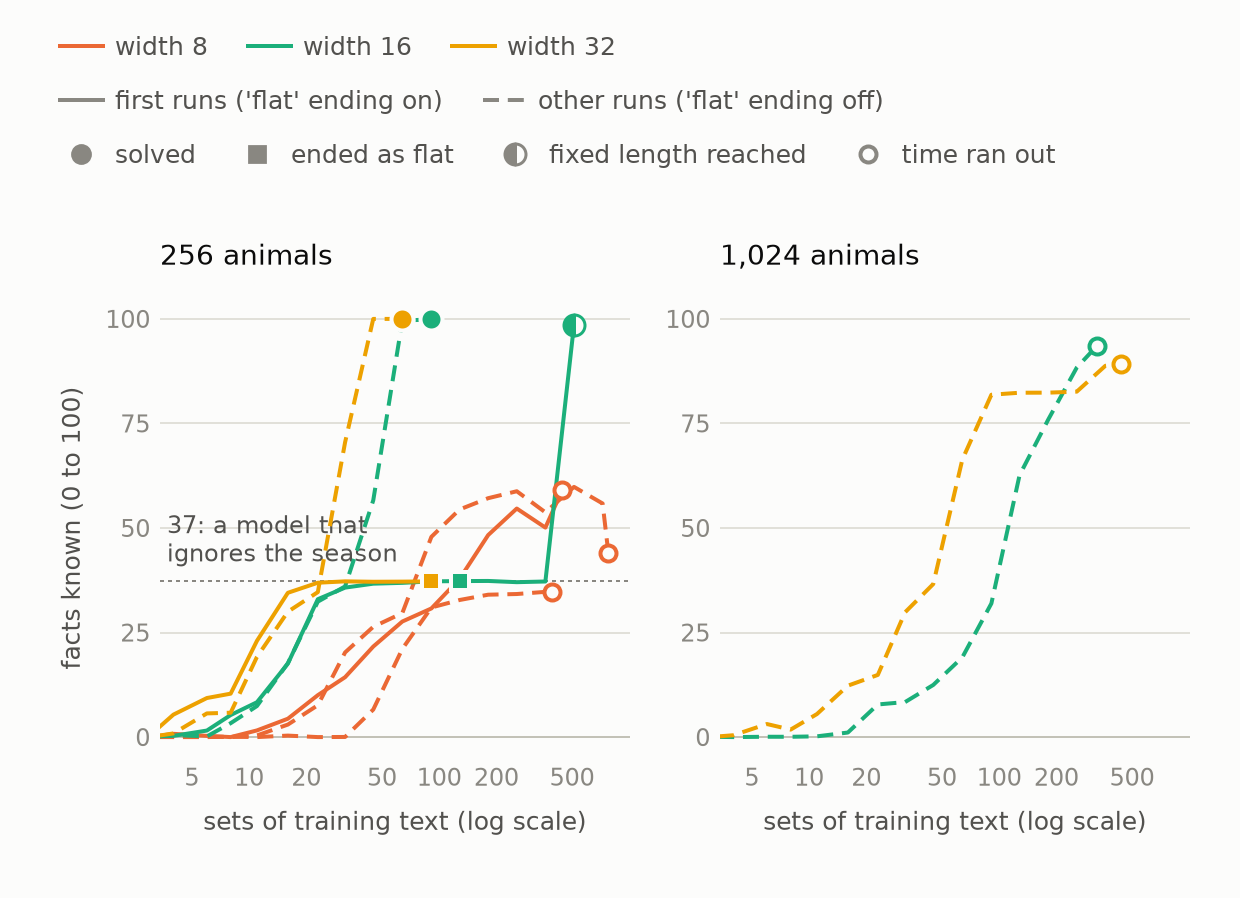
\includegraphics[width=0.68\textwidth]{figures/large_equal_x4.png}
\caption{The runs of table \ref{tab:large}, as training went on. Solid lines are the first
runs. The first run of width 16 is drawn as its exact retrace, which went on to 512 sets; the
square on it marks set 128, where the stopping test had ended it as flat. Dashed lines are the
other runs. The dotted line at 37 is the score of a model that ignores the season.}
\label{fig:large}
\end{figure}

\textbf{Whether a run stood still was a matter of chance.} Widths 16 and 32 made four different
attempts at the 256 animals. (The 512-set run retraced one of them exactly, so I do not count
it.) Two stood still at 37: the two first runs. Two went straight through and were solved
after 91 and 64 sets. The two runs of width 32 make the point most plainly. They started from
the same numbers and read the same text; for the second the computer was only set up
differently (it used a different number of its processors), which changes the last digits of
the arithmetic and nothing else. The first
was still standing at 37 when the test ended it at set 91. The second passed 37 without a
pause and knew every fact by set 45.

\textbf{Width 8 is the one place where your prediction may be showing.} By the rough guide it
would be 85\% full if it learned all 256 animals. That is under the limit, but the guide is
rough and comes from far larger models. Width 8 did not learn them in any of its three runs
(two repeats, the first of them run twice). In the first repeat it was at 59 after 445 sets;
run again, it kept shifting between 54 and 60 from set 128 to set 724 and was at 44 at its
last grading, set 776. In the second repeat it never came to use the season and stood between
33 and 35 from set 128 to its end. Width 16 reached 98.6 and 99.9 in the same two repeats, and
width 32 reached 100 in the one repeat it had. So here a model does do worse on more words, and wider models do better.

What width 8 knew is the most telling thing about it. The next figures are plain counts of
right answers in 100, not scores: guessing gives 25, and a model that ignores the season 53.
Both sets of figures come from the first repeat: its first run, and the same start run again
with the computer set up differently, which took a course of its own. When the first run
stopped, width 8 had 89 of the foods and 78 of the homes right, but only 57 of the colors and
54 of the waking times. When the second stopped, it had 93 of the homes and 81 of the waking
times, but only 34 of the foods and 25 of the colors. So the two runs held different pairs of
the four kinds of fact, and the second lost 12 points of score between its last two gradings.
It looks as if width 8 can hold about two of the four kinds at a time. That is what a model
that is too small would look like.

I still do not count it as support under our rule. The rule needs a run that ends flat by our
test, and none of the three did when I put the test to their saved scores afterwards. The two
runs of the first repeat never settled: their scores kept shifting by several points from one
grading to the next. The
second repeat did stand still, but its time ran out before it had stood still long enough for
the test to call it flat. And it was standing where we have seen models stand before: it took
no notice of the season, and other models went on from there in the end. But it is the best
lead of the night.

\textbf{On 1,024 animals,} which I had left out for lack of time, the cores that came free
allowed one long run each of widths 32 and 16. Both were still rising when their time ran out,
so they say nothing yet about limits. Width 16 was at 94 after 328 sets. Width 32 rose to 82
by set 91, stood there until set 256 while width 16 overtook it, and then moved again, to 89
at set 436. (At the end the homes were the one kind of fact it had not yet learned.)

\textbf{What this round says.} The verdict by the rule stays undecided: no run of width 8
ended flat, and where the first two parts of the rule did hold, for the first runs of widths
16 and 32, it was by a wrong ending. One caution about the lead at width 8: this round changed two things
at once. Each animal had four times as much to be remembered, and no fact could be answered
from the animal word alone any more, because the model had to put the animal and the season
together. These runs cannot tell me which of the two made the larger languages so much harder.

\section{Result 6: the smallest model}\label{sec:four}

You asked for width 4 to be kept in the record. I ran it on all four languages of the first
round and of the unequal-use round, three repeats each: 24 runs. By then many runs were sharing
the machine, so each went more than ten times slower than at the start of the night: in the 28
minutes (first-round languages) or 24 minutes (unequal use) that each had, it got through only
101 to 129 sets. One more run, on 16 animals, was trained for as long as the night allowed:
647 sets.

\textbf{Width 4 learned no facts.} Its score was 0 in 23 of the 24 runs and 0.3 in the other,
and it was still 0 after 647 sets in the long run. It did learn the shapes of the sentences. I
can tell from the finer measure of section \ref{sec:score}, how well a model predicts the next
word, on which lower is better. A model that knows how every sentence is built but no facts at
all scores 0.33 on it, and width 4 reached 0.36 by the end of the long run.

\textbf{How much these runs can bear.} In the first round, 112 to 129 sets are too few to
judge the two largest languages: width 8 had learned only part of them by then. Everywhere
else the comparison is fair. Width 8 knew every fact of the 16-animal language within 64 to
91 sets, and with unequal use it had a score of 77 or more on every language by set 91. Width 4 knew
nothing, and on 16 animals still nothing after 647 sets.

\textbf{This does not look like your idea at work.} Your idea says a model fails when it has
more to hold than fits. Width 4 fails with the fewest words. With 16 animals there are 128
bits to keep, and it has about 1,050 numbers in use (880 in its body and 43 rows of 4): about
6\% full by the rough guide. It seems to be too narrow to work at all. But I tried it for at
most 647 sets, and this night showed that a model can stand still for a long time and then
move, so even that is not proven.

\section{What this means for your idea}\label{sec:meaning}

Your idea has a starting claim and a prediction. The experiment bears on them differently.

\textbf{The starting claim is supported in these models.} A word's row holds most of what
the word means: section \ref{sec:probe} could read 70 to 97 in 100 of the animals' facts from
their rows alone, and animals that mean the same were given nearly the same row.

\textbf{The prediction was neither confirmed nor refuted, but there is a lead.} The
prediction is that a model of a given size does worse once it is given more words than fit.
Our rule looks for a model that comes to a stop at a lower score on more words while a bigger
model does better.
\begin{itemize}
\item With 8 bits per animal, no model ended up worse, even with 64 times as many animals. But
      by the rough guide no model was more than a little over one-third full, so the
      prediction was never put to the test.
\item With 32 bits per animal, widths 16 and 32 learned the 256 animals as well, though some
      of their runs first stood still for a long time. Width 8 did not learn them, in three
      runs on two repeats. That is the pattern of your prediction. It falls short of our rule
      because none of those runs ended flat by our test, and I cannot yet tell a model that is
      too small from one that is very slow.
\item Width 4 learned no facts on any language, so it says nothing about more words.
\end{itemize}

\textbf{Why adding words did not fill a model.} One part of the answer follows from how the
model is built: every animal comes with a row of its own. In the first round each added animal
brought 8 bits to be kept and, at width 8, 8 new numbers to keep them in: 1 bit per number,
half the rough limit, however many animals there are.

The other part is my guess. The number of words alone does not decide how big a model must be.
Two other things do. One is how much each word means, because that has to fit into the word's
own row, and a row has a fixed width. The other is how much there is to know about words
\emph{in combination} (here, an animal together with a season), because that is worked out in
the body, which all the words share. The 32-bit round speaks for this: width 8, with the
smallest rows of the three widths in that round, is the only one that did not learn the 256
animals. At width 8 a row has 8 numbers, which by the rough guide hold about 16 bits. Each
animal now has 32, so about half of what there is to know about it must be kept in the body.
For 16 animals that overflow takes about 5\% of the body; for 256 animals about four-fifths of
it, which by so rough a guide may be all the body can take. If that is right,
it is your idea in another form: the part of the model that all words share fills up as words
are added. It is a guess, and the next experiment should test it.

\textbf{What a larger vocabulary did cost: training.} With 8 bits per animal, 64 times as many
animals took about 6 to 8 times as many sets. With 32 bits per animal, 16 times as many animals
took 4 to 6 times as many sets when a run went straight through (widths 16 and 32: 91 and 64
sets against 16), and more than 20 times as many when it stood still (more than 362).

\textbf{A lesson about method.} During a stand-still a model looks exactly like one that has
reached its limit, and our stopping test was fooled by that on two occasions, the second
after I had already repaired it once. Your later suggestion, to give every model the same amount of text
and then compare, needs no judgment about when a model has finished. With amounts chosen
generously, I would use it in the next experiment.

\textbf{What this experiment cannot tell you.}
\begin{itemize}
\item It is a toy: the ``meaning'' of a word is four or sixteen facts, and the models are
      many thousands of times smaller than real ones. Nothing here carries over to large
      language models without further work.
\item The score is memory of facts. It says nothing about fluency or reasoning.
\item No score below 100 in this report is a proven limit. ``Flat'' and ``not finished'' both
      mean only that the model had not got further when its run ended.
\item Much of the 32-bit round rests on one or two runs for each setting, and that round
      showed how much one run can differ from the next.
\end{itemize}

\section{Everything I did that we had not agreed, and what is left}\label{sec:extras}

You gave me leave to make choices during the night and asked me to list them.

\textbf{Changes to the plan.}
\begin{enumerate}
\item The learning rate, the steadied copy of the model, and the extra conditions on the
      ``flat'' ending (section \ref{sec:changes}). Two smaller details were settled when the
      programs were reviewed: on the finer measure a change of less than 0.002 bits per word
      counts as no change, and a run is not asked whether it is flat at the extra grading made
      when its time runs out.
\item The 32-bit round was run although the first round did not meet the rule (you had told
      me during the night to run everything). Under the
      agreed procedure it was run on 16 and 256 animals only, and on 256 animals only once:
      when a long run showed that its ``flat'' endings were wrong, I dropped the repeats still
      to come and used the time for long runs with the ``flat'' ending switched off, on 256
      and then on 1,024 animals (section \ref{sec:round32}).
\item The time limit was 30 minutes per run in the first round, 15 in the 32-bit round (40 for
      one run) and 5 in the round with unequal use, to fit everything into one night. Width 4,
      on a crowded machine, had 28 and 24 minutes.
\item Until half past one, models were trained one at a time. After that the long runs,
      width 4 and the small checks ran side by side on separate processor cores, which got
      more done before morning but made each run slower. So I give sets, not minutes,
      wherever it matters.
\item Width 4 was run as you asked, but alongside the long runs and not after them, each run
      on a single slow core. That is why its runs are short (section \ref{sec:four}).
\item Before the first run I set aside a copy of the programs that train and grade the
      models, and every run of the night used that copy. Later corrections to the working
      version change nothing in how models are trained or graded, and none reached the runs.
\end{enumerate}

\textbf{Extra analyses and checks.} Three needed no new training: the look inside the word
table (section \ref{sec:probe}), the check on whether models use the season word (section
\ref{sec:round32}), and the comparison after equal amounts of text (section \ref{sec:equal}). Two small checks did need training. One is the check on
the steadied copy (section \ref{sec:changes}). The other is the side check we had planned:
does it matter that every model carries rows for all 1,024 animals even when its language has
only 16? I built width 32 with rows for its 16 animals and no others. It learned them in 23, 23
and 23 sets; with the full table it had taken 23, 16 and 23. So the idle rows changed nothing.

\textbf{Not done.} Of the 32-bit round as planned (four languages, widths 8 to 64, three
repeats), the 64-animal language, width 64, width 8 on 1,024
animals and every third repeat were not run at all; table \ref{tab:large} shows what was run
on the large languages. The word-table check for width 4. A check of width 6, which I started
and gave up for lack of time. And grading at finer steps, which we had talked about.

\textbf{What I would do next,} in this order.
\begin{enumerate}
\item \emph{Settle width 8 on 256 animals with 32 bits each:} three repeats, trained ten times
      as long, with width 16 beside it. If it reaches 100 it was only slow. If it does not, ``too
      small'' becomes more likely, though a stand-still can never quite be told from a limit.
\item \emph{Test your prediction in a model where a new word does not bring its own storage.}
      Give each animal a row of random numbers that training may not change. The row is then
      only a name tag, and everything the model learns about an animal must be kept in the
      body, which has a fixed size and is shared by all words. Then add animals until the body
      is full. There your prediction could succeed or fail far more clearly than here.
\item \emph{Compare after equal amounts of text, as you suggested,} and drop the stopping test.
      And \emph{find the smallest width that works} between 4 and 8.
\end{enumerate}

\textbf{Where everything is.} The programs are in the folder \s{air} (\s{README.md} explains
each one), the runs in \s{air/runs}, \s{air/runs\_long} and \s{air/runs\_extra}, and the
trial-run logs in \s{air/logs}.


\end{document}
